\documentclass{book}
\usepackage[fontset=windows]{ctex} % 使用 Windows 内置字体集,已包含中文字体支持
\usepackage{graphicx}
\usepackage{amsmath}       % 数学公式增强宏包
\usepackage{physics}      % 物理符号宏包
\usepackage{amssymb}       % 数学符号宏包
\usepackage{bm}            % 用于加粗数学符号

\usepackage{geometry}      % 页面布局宏包
\geometry{a4paper, margin=1in} % 设置页面大小和边距
\usepackage{fancyhdr}      % 页眉页脚宏包
\pagestyle{fancy}
\fancyhead{}               % 清除默认页眉
\fancyfoot{}               % 清除默认页脚
\fancyhead[L]{高等量子力学笔记} % 左侧页眉
\fancyhead[R]{ZhangX}     % 右侧页眉
\fancyfoot[C]{\thepage}   % 中间页脚显示页码
\usepackage{listings}      % 代码高亮宏包
\usepackage{xcolor}        % 颜色宏包
\lstset{                    % 设置代码高亮样式
    backgroundcolor=\color{lightgray!20}, % 背景颜色
    basicstyle=\ttfamily,   % 基本字体
    keywordstyle=\color{blue}, % 关键词颜色
    commentstyle=\color{green!50!black}, % 注释颜色
    stringstyle=\color{red}, % 字符串颜色
    numbers=left,           % 行号位置
    numberstyle=\tiny\color{gray}, % 行号样式
    stepnumber=1,          % 行号步长
    numbersep=5pt,         % 行号与代码间距
    showstringspaces=false, % 不显示字符串中的空格
    breaklines=true,       % 自动换行
    frame=single,          % 代码框
    tabsize=4,             % Tab 键宽度
    captionpos=b           % 标题位置
}
% \usepackage{unicode-math}  % Unicode 数学字体支持
% \setmathfont{Latin Modern Math} % 设置数学字体

\usepackage{bookmark}      % 先加载 bookmark
\usepackage{hyperref}      % 后加载 hyperref
\hypersetup{
    colorlinks=true,
    linkcolor=blue,
    bookmarksopen=true,
    pdfauthor={ZhangX},
    pdftitle={高等量子力学笔记}
}

\newenvironment{abstract}{\section*{README}}{\par}
\title{高等量子力学笔记}
\author{ZhangX}
\date{\today} % 自动插入当前日期

\begin{document}
\maketitle

\begin{abstract}
本文是作者基于《现代量子力学(第二版)》 (by 樱井纯)学习过程所记录的笔记。
\end{abstract}


\chapter{基本概念} % 中文章节标题
这本书摒弃了初等量子力学中按照历史发展顺序对量子力学一点一点介绍,而是从一个打破传统认知的实验开始。
\section{斯特恩-盖拉赫实验}
斯特恩-盖拉赫实验的前提认知是银原子中一个电子($5s$)的自旋(内禀的)提供了整个原子的磁矩,于是整个原子的磁矩满足,
\begin{equation}
    \bm{\mu} \propto \mathbf{S}
    \label{eq:1.1}
\end{equation}
其中,比例因子为 $\displaystyle \frac{e}{m_ec}$ 。磁矩在外加的磁场中会发生偏转。相互作用能为 $-\bm{\mu} \cdot \mathbf{B}$ ,
于是受力在 $z$ 方向分量的大小为
\begin{equation}
    F_z = \frac{\partial}{\partial z}\left(\bm{\mu}\cdot\mathbf{B}\right) 
    \simeq \mu_z \frac{\partial B_z}{\partial z}
    \label{eq:1.2}
\end{equation}
于是这个实验设计了一个局部不均匀磁场,这也是这个实验中创新的地方。按照经典力学的观点,原子取向是任意的,
那么 $\bm{\mu}$ 便无取向偏好,那 $\mu_z$ 便可以在 $[-|\bm{\mu}|, |\bm{\mu}|]$ 之间连续取值。形成一个弥散的斑痕,然而,事实并不如人们想的那样。
\begin{figure}[h]
    \centering
    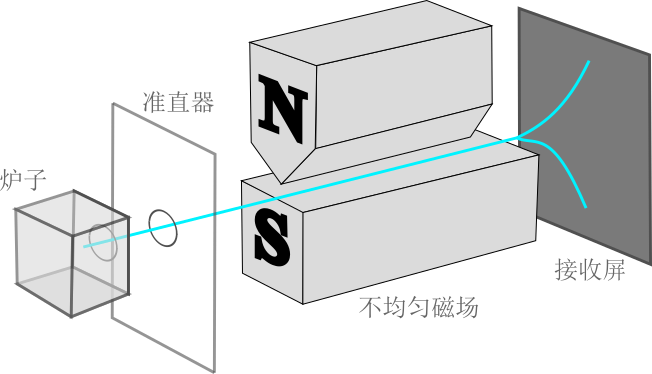
\includegraphics[width=0.5\textwidth]{img/斯特恩}
    \caption{Stern-Gerlach 实验}
    \label{fig:1.1}
\end{figure} 
实验的结果是如图 ~\ref{fig:1.1} 所示的两个点状图样。这就是空间量子化的宏观表现。然后我们设计进一步的实验,
\subsection{序列斯特恩-盖拉赫实验}
这一部分暂时不写,懒~(周一补齐)
\section{右矢、左矢和算符}
狄拉克发明的右矢和左矢,让计算变的简洁。//
\subsection{右矢空间}
为什么人们对于量子世界难以理解,就在于量子世界和经典世界对于物理量的描述方式是完全不同的。
在量子世界大门被推开的那一刻,人们是懵逼的,他们无法理解为什么一个粒子可以同时处在A和B两个位置上(实际并不是同时处于两个位置上,
只是两个位置上都有可能被测量到)。
随着实验和理论的推进,人们才意识到,量子是以概率幅存在的,那么就无法用一个数值去对其进行描述了。
那我们怎么描述,很简单,我们就用一个盒子把不同位置的概率幅装起来,然后有人问的时候,我们就把这个盒子打开给他看。
除了装位置的盒子,我们还有装动量的盒子,装能量的盒子,装自旋的盒子等等,然后我们把所有的盒子都放在一个大的盒子里。
这样就能完备的描述一个量子系统。这个盒子就是狄拉克定义的一个右矢。
\subsubsection{希尔伯特空间}




\end{document}